% Figure: gap closed against the promised excess G, for the joint winner, the
% constant-shape ablation and the two comparators, at the three load levels.
% Every coordinate below is a cell of Table~\ref{tab:guard} (column "Gap closed",
% rows Guard(G) / Guard-fixed(G) / Fixed(G) / Skip(G) at G = 300, 600, 1200 s),
% which comes from outputs/paper_tables/tab_guard.tex.  No new computation.
\begin{figure}[htbp]
\centering
\resizebox{\textwidth}{!}{%
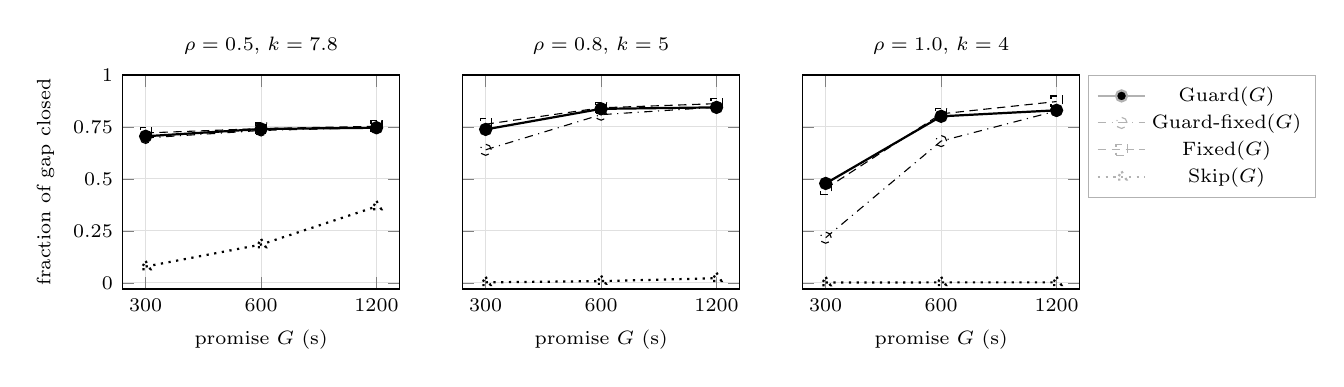
\begin{tikzpicture}[font=\footnotesize]
\pgfplotsset{
  gapaxis/.style={
    width=5.1cm, height=4.3cm,
    symbolic x coords={300,600,1200}, xtick=data,
    xlabel={promise $G$ (s)}, ymin=-0.03, ymax=1.0,
    ytick={0,0.25,0.5,0.75,1}, grid=major, grid style={black!12},
    tick label style={font=\scriptsize}, label style={font=\scriptsize},
    title style={font=\scriptsize, yshift=-2pt},
  },
}
\begin{axis}[gapaxis, ylabel={fraction of gap closed},
             title={$\rho = 0.5$, $k = 7.8$}, name=p1]
  \addplot[mark=*,thick]            coordinates {(300,0.705) (600,0.740) (1200,0.746)};
  \addplot[mark=o,dash dot]         coordinates {(300,0.697) (600,0.733) (1200,0.747)};
  \addplot[mark=square,densely dashed] coordinates {(300,0.721) (600,0.742) (1200,0.753)};
  \addplot[mark=triangle,dotted,thick] coordinates {(300,0.078) (600,0.184) (1200,0.367)};
\end{axis}
\begin{axis}[gapaxis, title={$\rho = 0.8$, $k = 5$},
             at={(p1.east)}, anchor=west, xshift=8mm, name=p2, yticklabels={}]
  \addplot[mark=*,thick]            coordinates {(300,0.738) (600,0.837) (1200,0.844)};
  \addplot[mark=o,dash dot]         coordinates {(300,0.640) (600,0.809) (1200,0.845)};
  \addplot[mark=square,densely dashed] coordinates {(300,0.763) (600,0.842) (1200,0.862)};
  \addplot[mark=triangle,dotted,thick] coordinates {(300,0.002) (600,0.008) (1200,0.022)};
\end{axis}
\begin{axis}[gapaxis, title={$\rho = 1.0$, $k = 4$},
             at={(p2.east)}, anchor=west, xshift=8mm, yticklabels={},
             legend style={font=\scriptsize, at={(1.03,1.0)}, anchor=north west,
                           draw=black!30, row sep=-1pt}]
  \addplot[mark=*,thick]            coordinates {(300,0.478) (600,0.801) (1200,0.830)};
  \addlegendentry{Guard($G$)}
  \addplot[mark=o,dash dot]         coordinates {(300,0.217) (600,0.682) (1200,0.827)};
  \addlegendentry{Guard-fixed($G$)}
  \addplot[mark=square,densely dashed] coordinates {(300,0.453) (600,0.813) (1200,0.872)};
  \addlegendentry{Fixed($G$)}
  \addplot[mark=triangle,dotted,thick] coordinates {(300,0.001) (600,0.002) (1200,0.002)};
  \addlegendentry{Skip($G$)}
\end{axis}
\end{tikzpicture}}
\caption{Original source-clock scores (optimistic reference): what each budget shape keeps of the FCFS-to-SJF gap as the promised
excess $G$ is relaxed. Every point is a ``Gap closed'' cell of
Table~\ref{tab:guard}; the intervals are in that table and are omitted here.
All four policies carry the same promise at a given $G$, since the promise
depends on the cap alone. The gap between Guard($G$) and its constant-shape
ablation opens where the promise is tight and the load is high and closes
elsewhere; counting positions rather than work (Skip) collapses at the two higher
loads; Fixed($G$), which spends the whole cap, buys its gap with harm the
selection rule rejects.}
\label{fig:gapvsg}
\end{figure}
